%%
%% This is file `example/ch_intro.tex',
%% generated with the docstrip utility.
%%
%% The original source files were:
%%
%% install/buptgraduatethesis.dtx  (with options: `ch-intro')
%% 
%% This file is a part of the example of BUPTGraduateThesis.
%% 

\chapter{原型系统设计与实现}
本章主要对本课题的算法模型实际落地的原型系统设计与实现进行了介绍,主要包括需求分析,系统设计,系统功能测试三部分内容,由于系统设计不是本课题的重点,因此仅对本课题在原型系统的开发中承担的部分进行介绍。

\section{引言}
\label{sec:sys_intro}
本章系统旨在立足法官判案的核心需求,基于裁判文书和法院案卷等司法案例数据,运用大数据、机器学习等信息技术,构建司法类案推送系统,实现司法知识表示系统化、类案匹配立体化、类案推送个性化,与审判业务系统深度融合,与法官日常办案无缝对接,为人民法院统一裁判尺度、提升司法权威和公信力提供有力的技术支撑。
\section{需求分析}

% 作为司法裁判改革所关注的核心问题,“同案不同判”抑制是影响司法公信的主要原因之一。针对我国国情,造成裁判尺度不统一的成因主要包括四个方面:
% \begin{itemize}
%     \item 1)案情相同,但是当事人举证不同:较好地举证有助于诉讼请求获得支持,反之,举证不能则可能导致败诉;
%     \item 2)法律的变迁与法律规范之间的冲突:法律体系内的冲突和矛盾导致司法者在适用法律上的选择性更强,进而为裁判结果的不统一创造了条件;
%     \item 3)参与决定裁判结果的人员认识不一:目前司法制度体系造成判决是法官、合议庭、法院领导的共同研究决定,容易造成法律适用、事实认定、自由裁量权上的观点和标准不同;
%     \item 4)法官认识的阶段性:法官自身知识体系、素质存在认识局限性,随着认识的深入和透彻,造成新的裁判不同于之前的裁判结论。针对以上成因,最高人民法院以及地方各级法院已经在大力度地推进相关工作,比如最高人民法院已经开始发布指导案例,来统一同类案件裁判标准;深化司法公开,进行信息化建设,促使裁判者更加“慎断”。
% \end{itemize}

“同案不同判”是目前司法领域面临的一个核心问题,即针对相似类型的案件,法官的裁判结果不同,造成这一情况的原因包括以下几点:
\begin{itemize}
    \item 各级法院法官的受教育程度不同,审判案件数量不同,导致对案情理解有所不同,造成不同的判决结果。
    \item 案情描述包括事实描述和证据两部分,针对同样的事实描述,由于证据的不同,可能导致完全不一样的裁判结果。
    \item 由于不同年代有不同的时代背景,因此,不同时代针对同一事件的看法观点不同,因此法律在不同时代下规定也有所不同,法律体系中现有规定由重叠的部分,因此,法官在进行量刑判决的时候有很大的选择空间,导致采用不同法规时导致不同的裁判觉过。
\end{itemize}

% 因此,立足这几个法官判案的核心需求,基于裁判文书和法院案件卷宗等司法案例数据综合运用大数据、机器学习等信息技术,构建司法类案推送系统,实现司法知识表示系统化、案情画像精细化、类案匹配立体化、类案推送个性化。与审判业务系统深度融合,与房管日常办案无缝对接,为人民法院统一裁判尺度、提升司法权威和公信力提供有力的技术支撑。

因此,针对目前司法领域的这个主要问题,利用法院电子信息化多年积累的裁判文书和司法数据,结合大数据,人工智能等相关技术,构建司法案例检索系统,实习立体化的类案匹配。


\section{系统设计}

本节主要介绍了原型系统的整体设计,首先介绍了原型系统的功能设计,之后介绍了数据库的设计。

\subsection{系统功能设计}
% 作为智慧司法的重点应用,司法类案推送是统一裁判标准、推进司法公正的重要手段。因此,亟需在司法大数据基础上,通过系统性攻关案件要素提取、案情画像构建、案情语义匹配、个性化类案推送等关键技术,构建高效可靠的类案自动推送系统,解决法官判案日常需求中的痛点问题,提高案件受理、审判环节的智能化水平,推动司法公平正义。系统整体设计如图~\ref{fig:sys_main}所示:

本原型系统立足目前司法领域的核心需求,种族要设计了案情要素提取,类案语义匹配,类案检索以及法条推荐四部分核心功能,为法官判案进行司法辅助,实现司法判决的一致性,提高法官办案效率,为民众提供法律咨询,提供司法领域智能化水平,实现司法公正。本原型系统的整体功能设计如图\ref{fig:sys_main}:
\begin{figure*}[htbp]%[htbp]
    \centering
    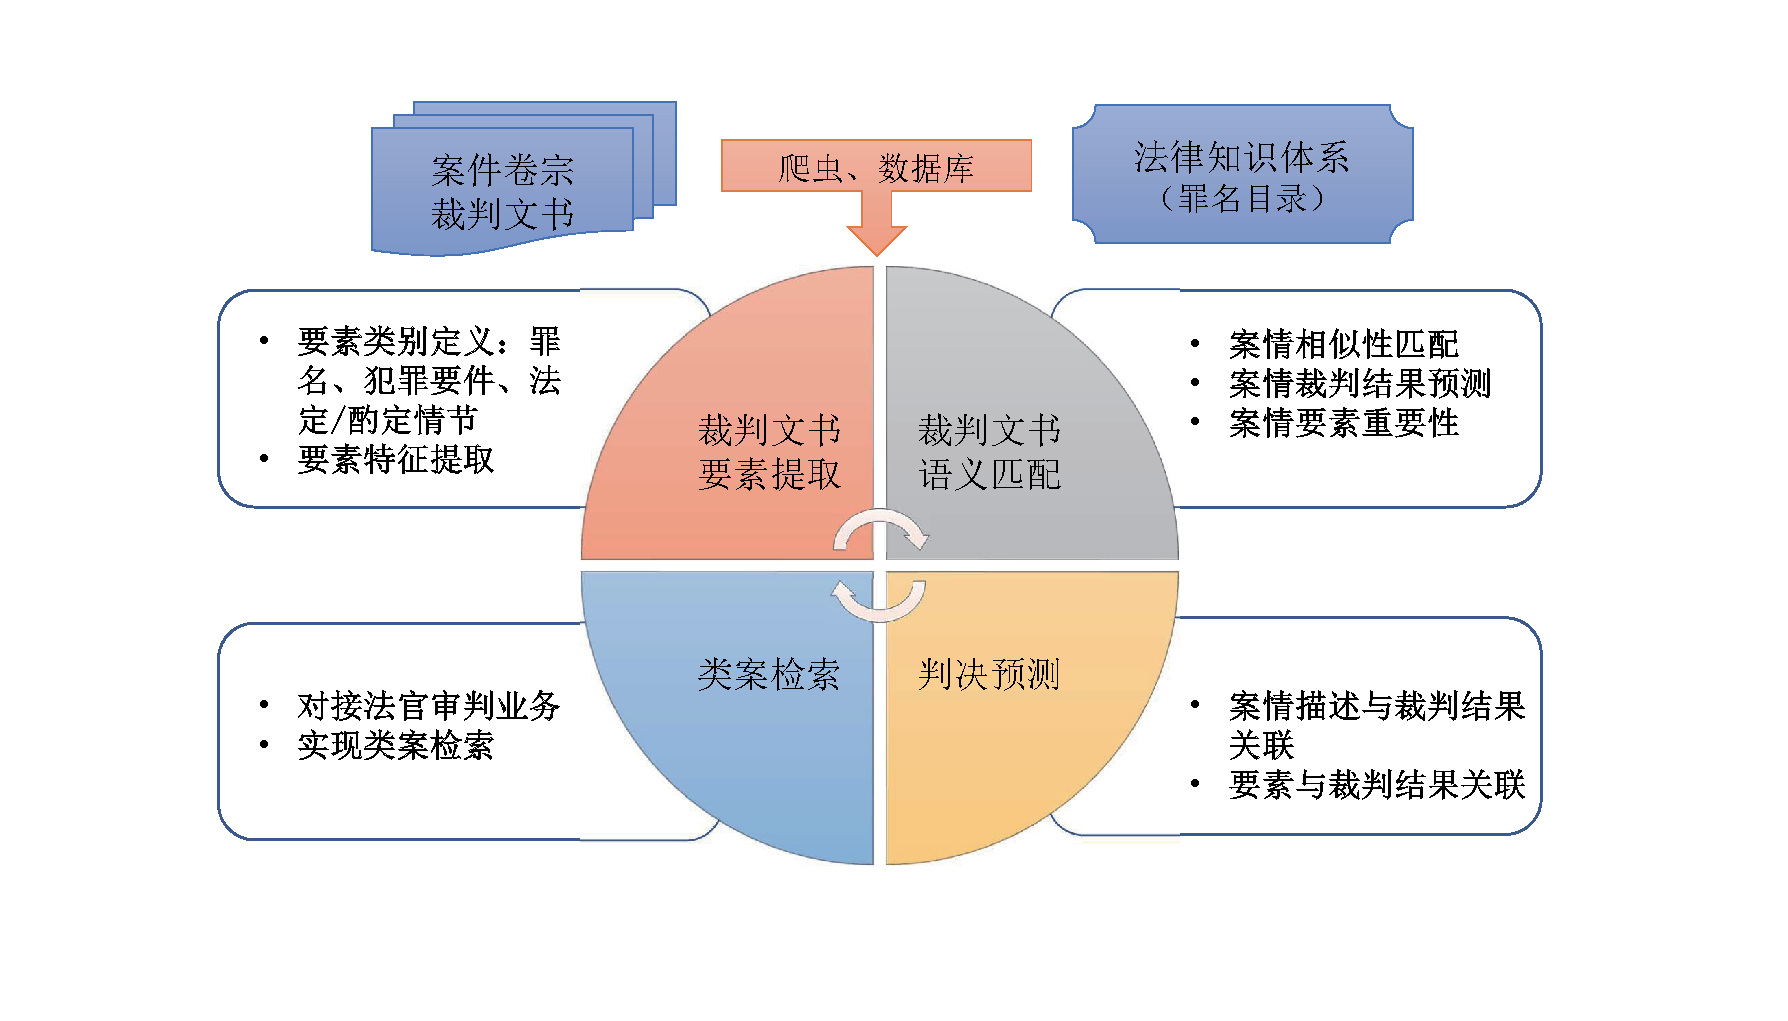
\includegraphics[scale=0.5, clip=true]{./sources/sys_main.eps}
    \caption{\label{fig:sys_main}案情要素特征样例图}
\end{figure*}



\subsubsection{裁判文书要素提取功能}
% 根据我国司法理论,任何一种犯罪的成立都必须具备四个方面的构成要件,即犯罪客体、犯罪客观方面、犯罪主体和犯罪主观方面。由此,本研究内容旨在对案件的若干案件要素特征进行定义,通过专家标注和自动规则学习方法,可以对案件文书/卷宗的要素特征进行实例化,从而获得案件的要素特征表示,如下图所示~\ref{fig:sys_element_demo}:

裁判文书是法官在审理案件之后,整理得到的书面报告。目前最高人民法院已经积累了大量这方面的数据,其中包含了很多有价值的信息,同时也是本课题研究的数据基础。本课题通过规则以及半监督学习的方式对文书进行处理,得到案件要素特征,案件要素特征样例如图~\ref{fig:sys_element_demo}:
\begin{figure*}[htbp]%[htbp]
    \centering
    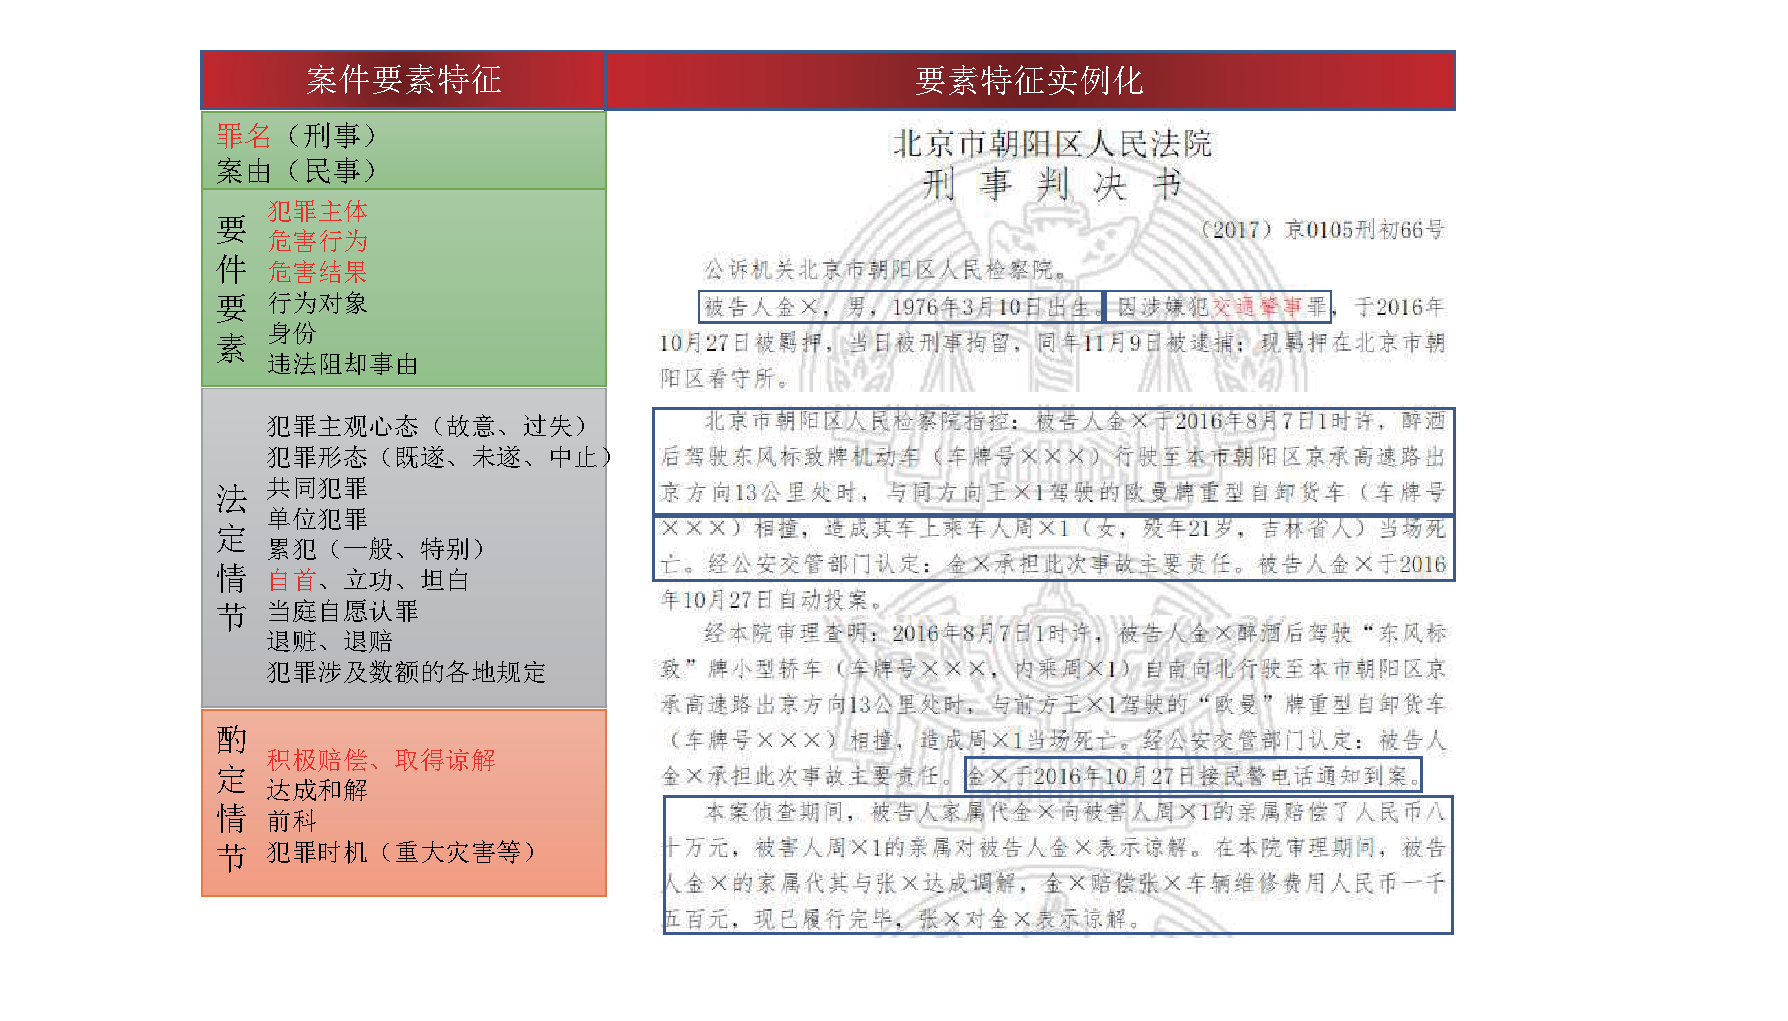
\includegraphics[scale=0.5, clip=true]{./sources/sys_element_demo.eps}
    \caption{\label{fig:sys_element_demo}案情要素特征样例图}
\end{figure*}

% 具体的,对于形事案件,与类似案件相关的要素特征包括罪名或案由、犯罪要件要素、法定情节、酌定情节等。其中,犯罪要件要素包括: 犯罪主体、危害行为、 危害结果、 行为对象、 身份、 违法阻却事由;法定情节包括: 犯罪主观心态(故意、过失) 、 犯罪形态(既遂、未遂、中止) 、 共同犯罪、 单位犯罪、 累犯(一般、特别) 、 自首、立功、坦白、 当庭自愿认罪、 退赃、退赔、 犯罪涉及数额的各地规定等;酌定情节包括: 积极赔偿、取得谅解、 达成和解、 前科、 犯罪时机(重大灾害等) 。 类似的,我们也可以定义对于民事案件的类案相关要素特征。

% 基于给定的案件要素特征,进行信息提取,即根据预先定义的模版,从文书中提取出特定的信息并形成结构化数据, 形成对裁判文书信息内容的结构化处理,获得案件的要素特征表示。


具体地,案件要素特征主要包含罪名,案件要素,法定情节,酌定情节四方面内容。案件要素针对犯罪中的主要行为人以及主要情节进行规定;法定情节是法律规定的一些情节,针对被告人的一些犯罪主观状态进行规定,用于作为加重刑罚和减轻刑罚的依据。酌定情节是由司法机关自行决定的一些对于被告人加重刑罚以及减轻刑罚的依据。

基于这些案件要素特征,本课题制定相应的规则模板,对裁判文书的相应内容进行定义。本课题采用基于规则的信息抽取方法,对司法领域要素信息进行抽取。基于规则的信息抽取方法假设人们在表达某些信息时经常使用某种特定的语言模式,通过捕获和学习可靠的信息识别和提取规则,可以将学习的模式与所检查的文本相匹配,一旦找到匹配,则触发提取动作将匹配的文本片段转移到目标结构中。

典型的可训练信息抽取系统遵循包括语言预处理,学习和应用阶段的流水线架构,如下图所示\ref{fig:sys_element_tech}。

\begin{figure*}[htbp]%[htbp]
    \centering
    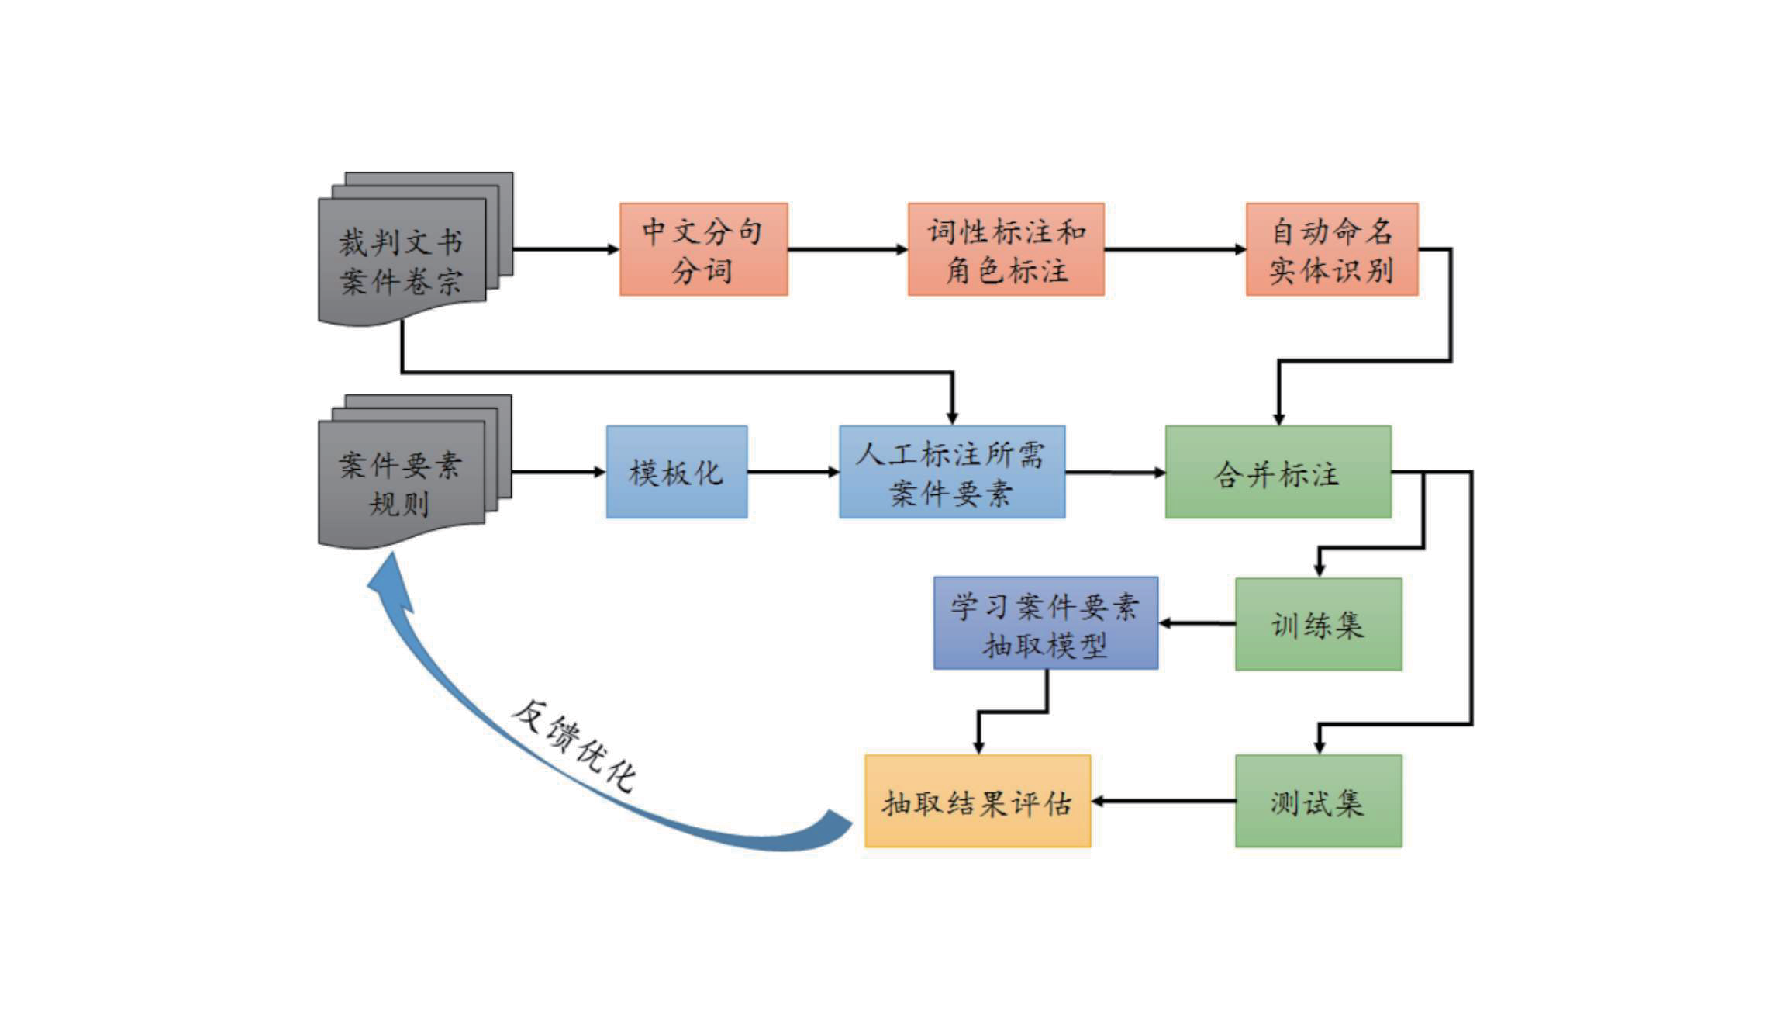
\includegraphics[scale=0.5, clip=true]{./sources/sys_element_tech.eps}
    \caption{\label{fig:sys_element_tech}裁判文书要素特征提取功能设计图}
\end{figure*}

具体的,通过人工标注案件要素特征对裁判文书进行编码,作为初始的要素提取模型;结合中文分词、词性标注、命名实体识别等基础词法分析方法,初始模式可以捕获上下文、词汇和语言信息,通过模板匹配算法将模式与相应的提取动作相关联来构建初始规则,该提取动作将特别指出的提取片段传送到目标结构中。

初始规则构成了学习过程开始时的规则库。将规则库用于训练语料库,并将其提取结果与人工标注进行比较,计算信息提取精度。高精度的提取规则将作为正确规则添加到正确规则集中。生于的规则进入拒绝的规则池中。通过规则矫正产生更多可靠的广义规则,以建立应用领域的良好覆盖。

在原型系统中,采用正则匹配方法和iepy\footnote{https://iepy.readthedocs.io}作为工具用于信息抽取。本课题所用自有数据集均通过信息抽取进行收集,通过对案情描述相应段落的首尾特点,提取裁判文书中的案情描述段落,裁判结果,对应法条等结果。

% \subsubsection{案情画像构建功能}
% 本原型系统旨在按照案件审判的一般逻辑依据,从使用法律、案件事实和裁判结果三个维度对案情进行精细化画像构建,为后续语义匹配奠定基础。具体的,从各类司法案件中,通过裁判文书可以建立案件要素特征到裁判罪名和量刑之间的关联关系。基于海量文书中的这种对应关系,运用关联规则分析挖掘方法,可以针对离散的案件要素进行有机重构,从而获得要素特征与最终裁判罪名,涉及法条,量刑确定之间的关联关系,基于知识图谱技术,构建司法知识体系,用于后续案情匹配任务,该模块如图~\ref{fig:sys_picture}所示:


% 该模块不是本课题研究的重点,故不进行详细描述。
\begin{figure*}[htbp]%[htbp]
    \centering
    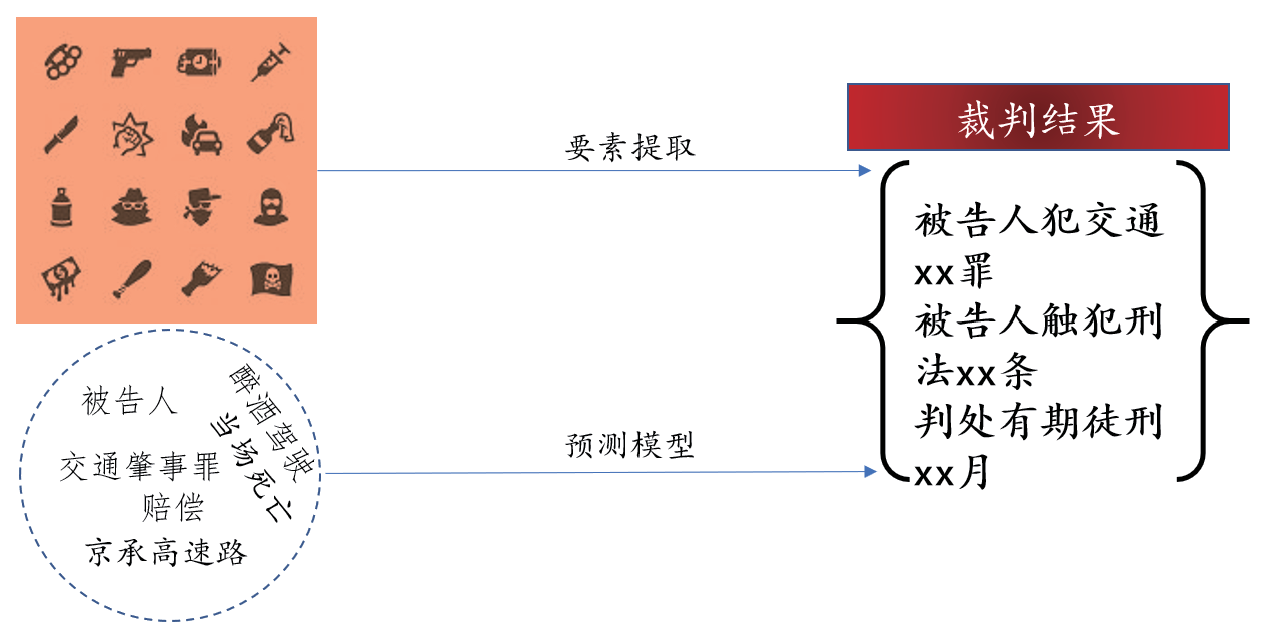
\includegraphics[scale=0.5, clip=true]{./sources/sys_picture.eps}
    \caption{\label{fig:sys_picture}案情画像功能设计图}
\end{figure*}


\subsubsection{裁判文书语义匹配功能}
\label{sec:sys_content}
类似裁判文书的概念内涵包括三层含义,即,犯罪事实基本一致、使用法律基本一致、裁判结果基本一致。因此,类案匹配应当以“法条”,“罪名”和“量刑”为首要依据,以“案件要素要件、法定或酌定情节”作为进一步依据。

裁判文书语义匹配功能主要针对犯罪事实基本一致进行匹配,即从案情描述角度进行计算。本原型系统利用案情描述与裁判依据(法条)预测模型为基础,构建案情的语义相似度度量方法。如图\ref{fig:sys_similarity}所示:
\begin{figure*}[htbp]%[htbp]
    \centering
    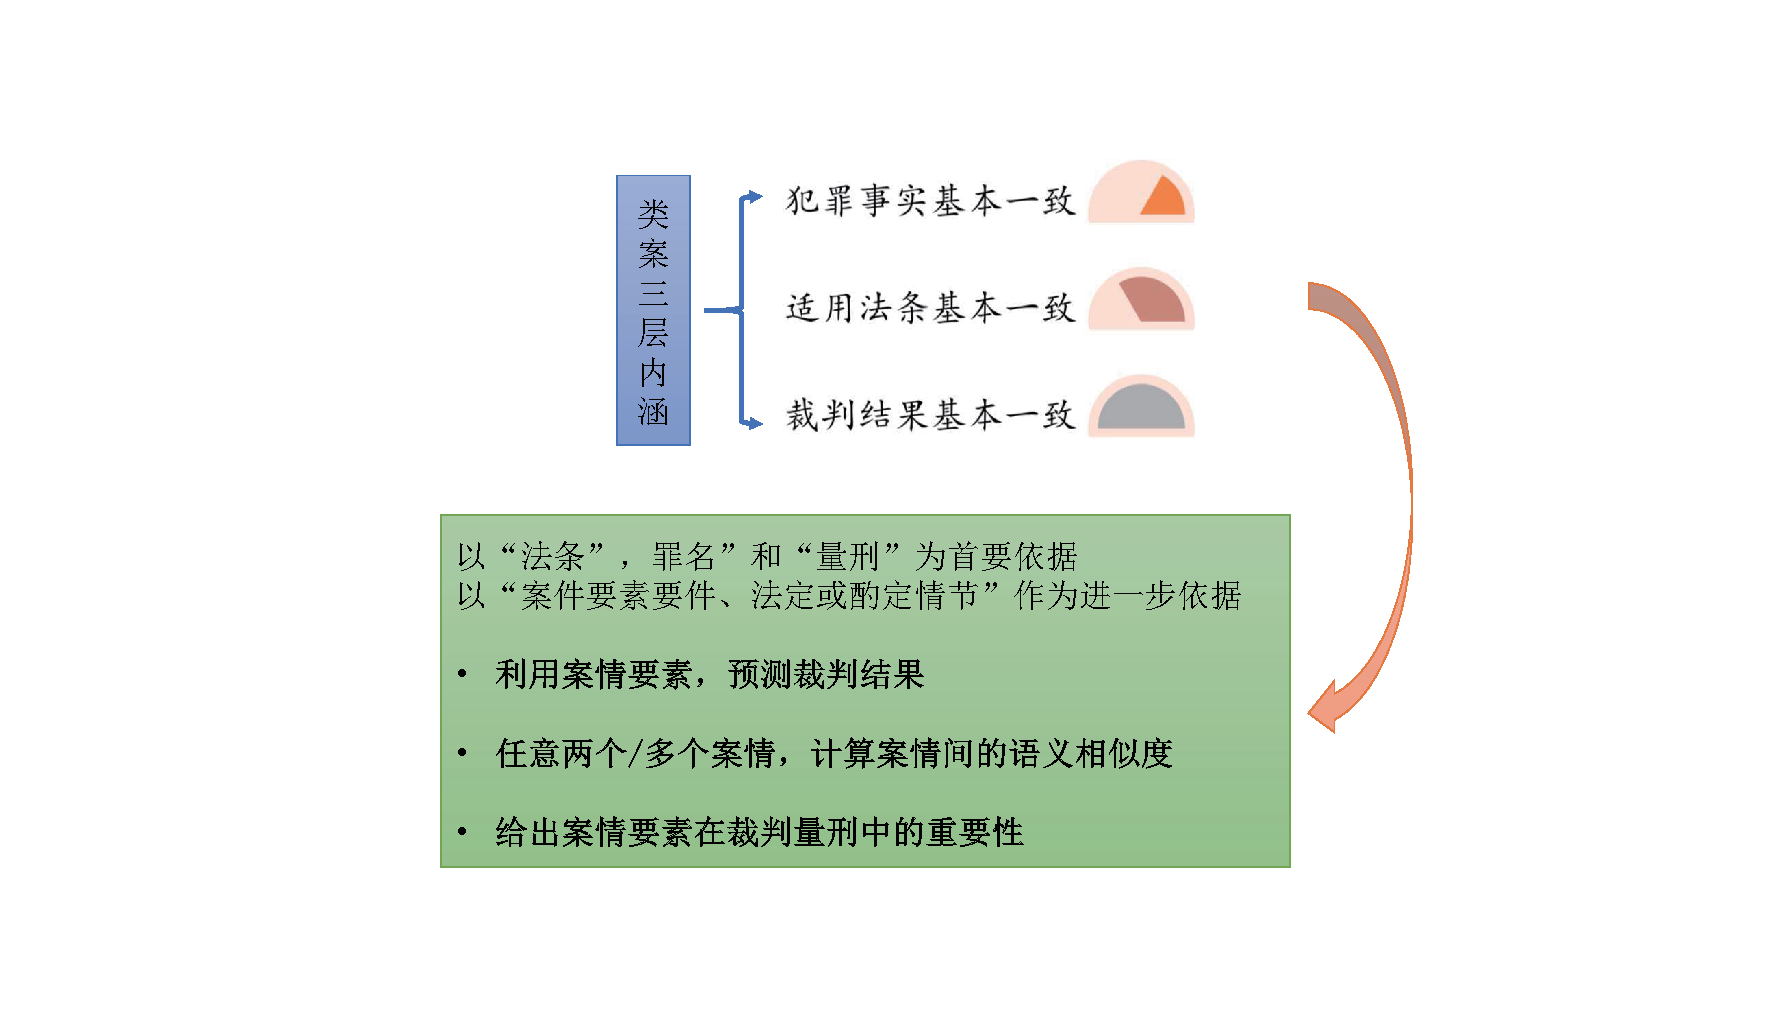
\includegraphics[scale=0.5, clip=true]{./sources/sys_similarity.eps}
    \caption{\label{fig:sys_similarity}语义相似度计算功能设计图}
\end{figure*}

目前的案情相似度计算方式包括:
\begin{itemize}
    \item 1)基于关键词匹配算法:利用关键词进行检索,使用基于tf-idf的语言模型计算查询与文书的相关性
    \item 2)基于主题的匹配算法:利用裁判文本语料库,训练获得重要的主题,并计算查询与文本的相似度
    \item 3)基于词向量的匹配方法:利用裁判文书语料库,训练获得词向量,并利用min-max pooling方法计算查询与文书的语义相似度
    \item 4)基于裁判过程的匹配算法:依据案件特征与裁判结果对应关系,训练裁判结果预测模型,并根据文书之间的裁判逻辑过程计算语义相似度
\end{itemize}

这四种计算方法,由于时间复杂度有差异,算法精度差异,根据需求不同,用于不同情况下的语义相似度计算。结合以上几种方法构建语义相似度计算框架,计算流程如图~\ref{fig:sys_similarity2}:
\begin{figure*}[htbp]%[htbp]
    \centering
    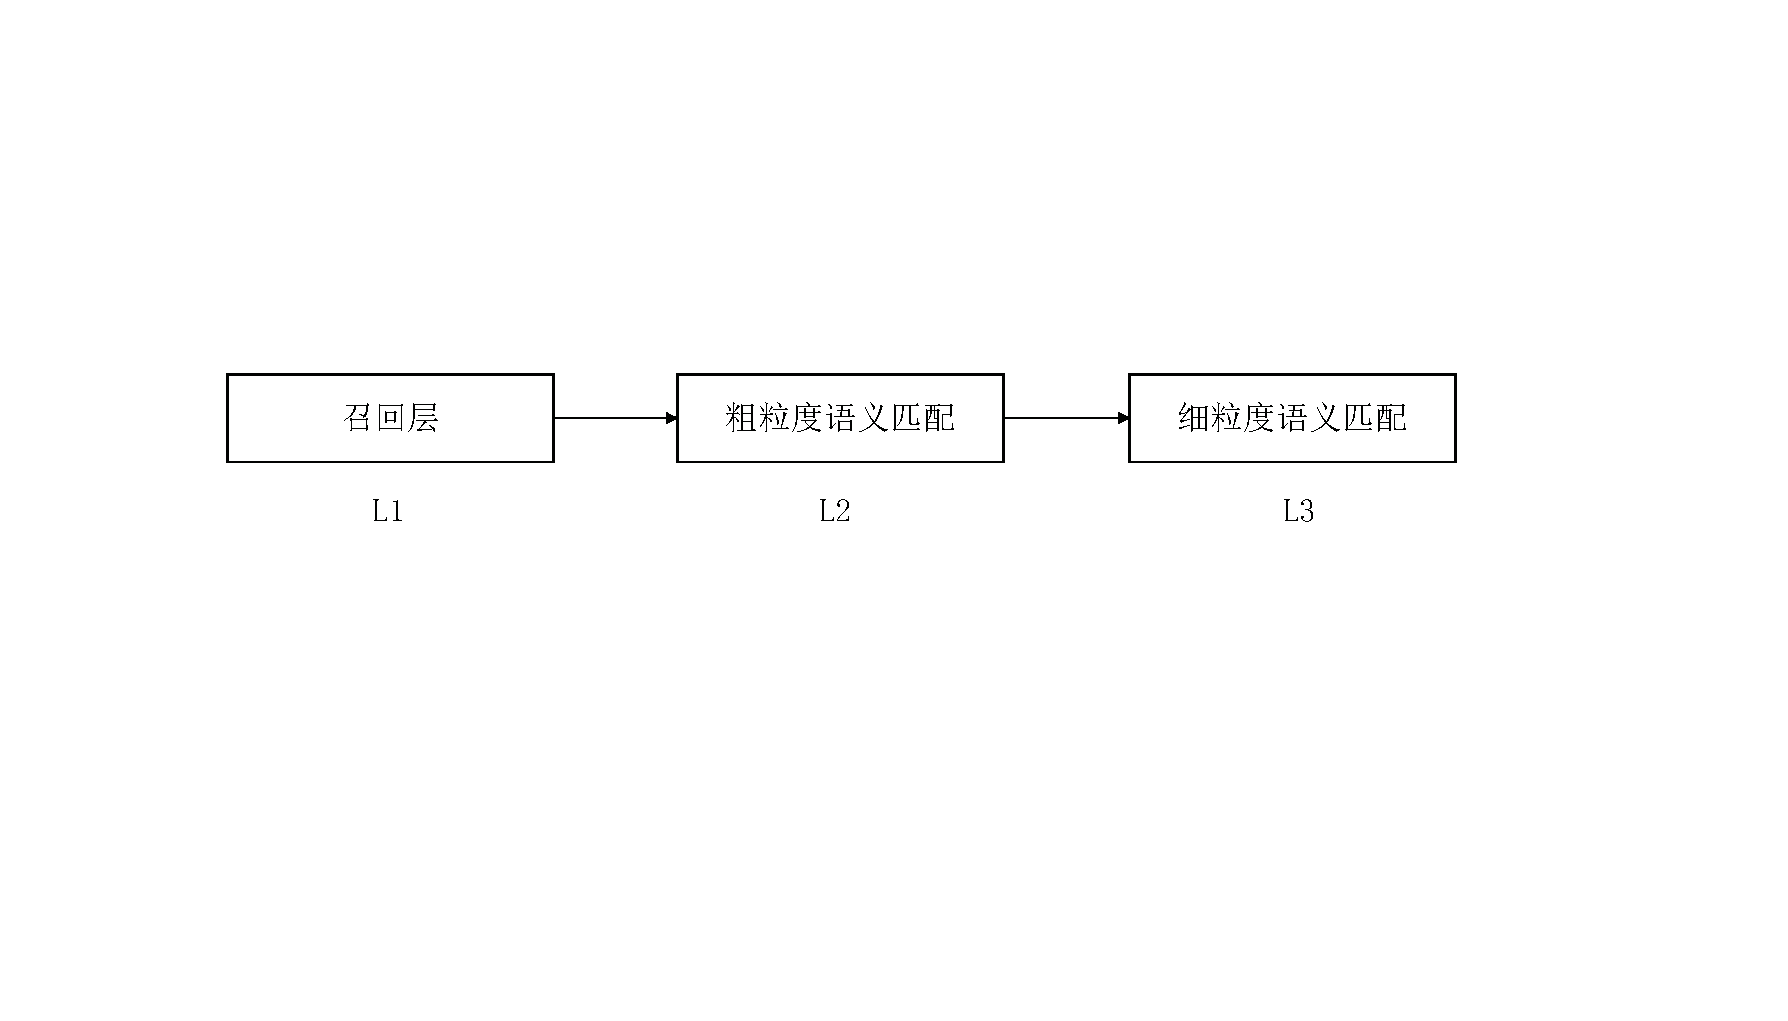
\includegraphics[scale=0.5, clip=true]{./sources/sys_similarity2.eps}
    \caption{\label{fig:sys_similarity2}语义相似度计算流程图}
\end{figure*}

裁判文书语义相似度计算由三层组成,三层分为称为召回层,粗匹配层,细粒度匹配曾。根据三层的不同分工,采用不同的案情相似度计算方法。具体地,总结如下:
\begin{itemize}
    \item 关键词匹配算法由于速度快,并且能有效得到与查询文字上相关的信息,因此,作为候选样例召回方法,从大量裁判文书中召回与用户查询需求基本相关的若干文档,位于L1层次。
    \item 基于主题的匹配算法和基于词向量的匹配算法,引入了一定的语义信息,位于L2层,对L1召回的裁判文书中进一步,得到与用户查询有基本语义关联的文档,进一步缩减文档数量。
    \item 利用本课题第三章以及第四章提出的模型进行分类,旨在学习案件审理逻辑。由于深度学习模型计算复杂度高,因此作为最后一层L3层的相似度计算方法,在文档数量相对较少时对语义相似度进行匹配。
\end{itemize}



% 类似裁判文书的概念内涵包括三层含义,即,犯罪事实基本一致、使用法律基本一致、裁判结果基本一致。因此,类案匹配应当以“法条”,“罪名”和“量刑”为首要依据,以“案件要素要件、法定或酌定情节”作为进一步依据。

% 具体地,案件要素特征主要包含罪名,案件要素,法定情节,酌定情节四方面内容。案件要素针对犯罪中的主要行为人以及主要情节进行规定;法定情节是法律规定的一些情节,针对被告人的一些犯罪主观状态进行规定,用于作为加重刑罚和减轻刑罚的依据。酌定情节是由司法机关自行决定的一些对于被告人加重刑罚以及减轻刑罚的依据。

% \subsubsection{个性化推送功能}
% 本原型系统采用个性化信息检索基础框架,构建历史案例知识库索引;针对包括要素标签、样例文书、案情描述等在内的不同形式的信息需求,构建共享编码器,提供统一的查询意图形式化编码;基于案情语义匹配功能模块,与案例知识库进行案情相似性匹配和裁判结果相似性匹配,综合两者匹配度获得初步的类案推荐列表;最终根据法官实际个性化需求,一句时间、地域、特定案件类型等对推荐列表进行个性化重排序,并返回给法官支撑其审判业务。其过程如图~\ref{fig:sys_recomm}:
\subsubsection{类案检索功能}
本原型系统采用全文检索系统作为基础框架,利用



\begin{figure*}[htbp]%[htbp]
    \centering
    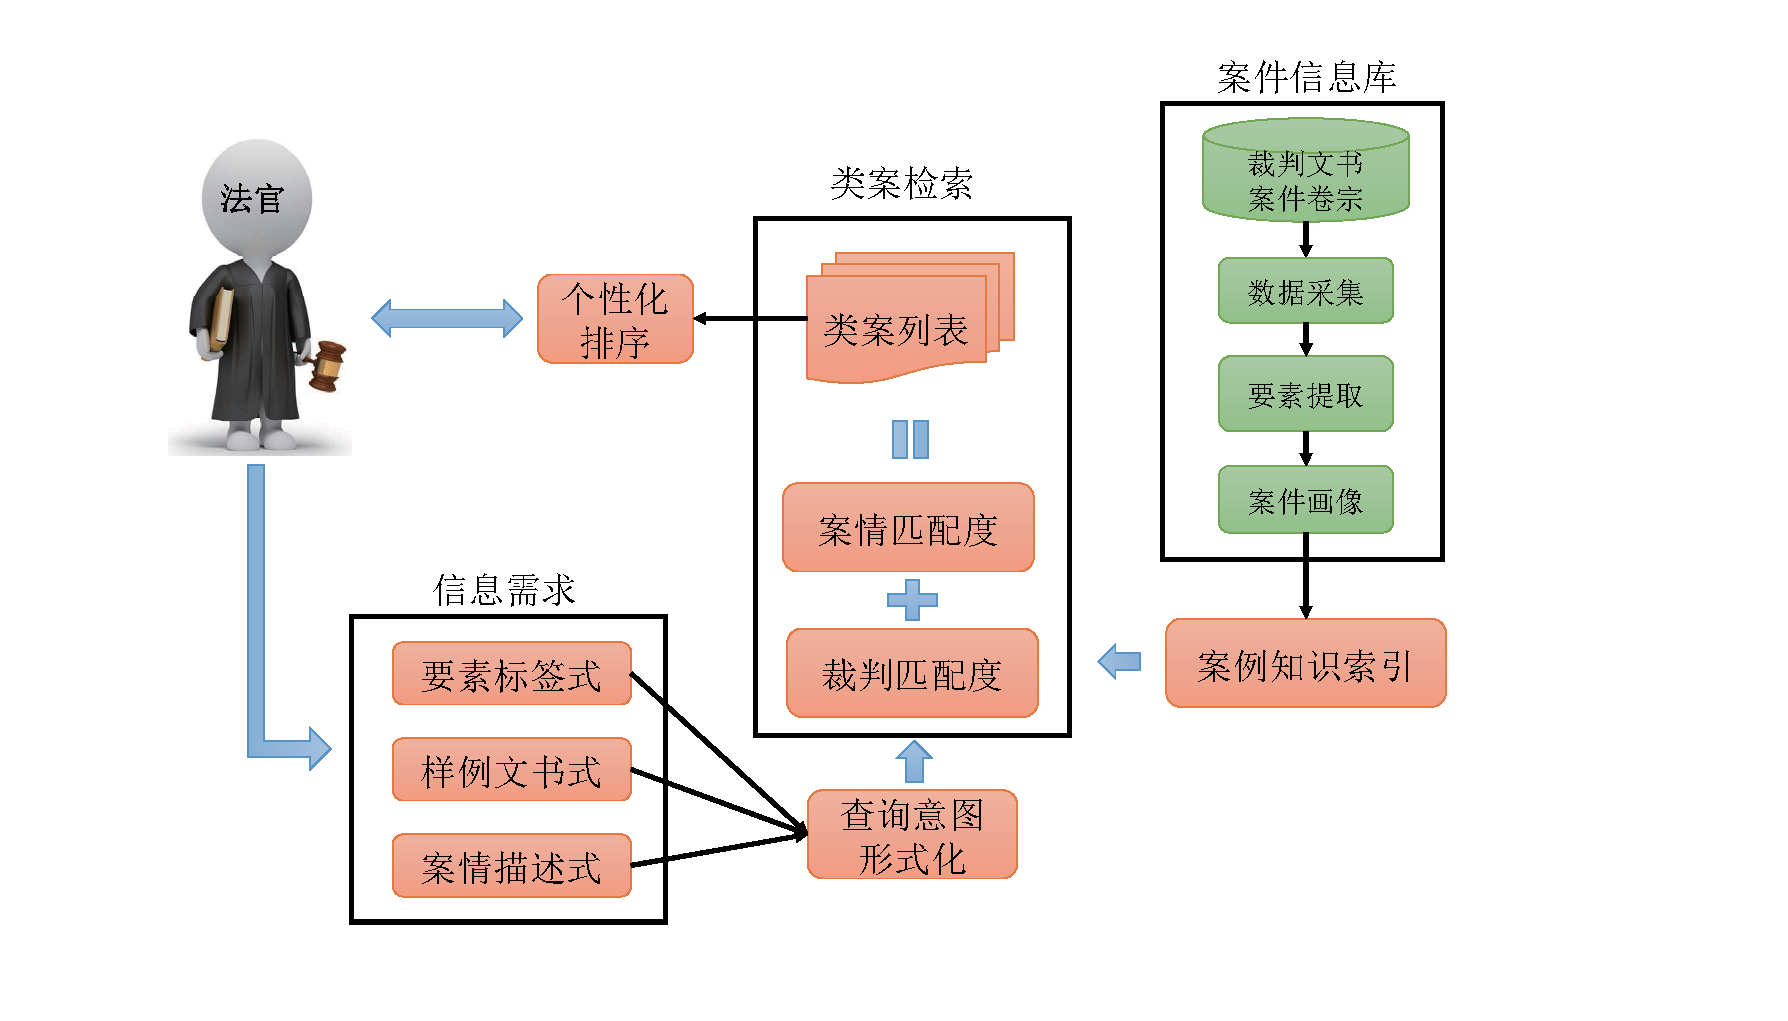
\includegraphics[scale=0.5, clip=true]{./sources/sys_recomm.eps}
    \caption{\label{fig:sys_recomm}个性化推荐功能设计图}
\end{figure*}


个性化类案推送系统通过获取与法官相关的特征信息,构建用户模型,并运用这些特征信息参与信息检索,帮助获得与法官偏好更贴切的个性化信息,同时引入反馈流程提供更加准确和友好的类案推送服务。 用户偏好学习拟采用如下技术途径: 通过法官的地域、领域等属性,进行智能排序; 通过用户对检索结果的显式反馈意见调整、修改用户偏好;通过用户行为监测模块对用户行为进行点击等行为分析挖掘,推导出用户偏好。

本部分不是本课题的研究重点,此处不进行详细介绍。


% \subsection{数据库设计}

\section{系统功能测试}
本节主要对原型系统功能进行测试,主要包括类案检索功能测试,判决预测功能进行测试。
\subsection{类案检索功能测试}
类案检索通过用户输入案情信息,为法官和普通用户推送相关案列,其演示结果如图
~\ref{fig:sys_search}:
\begin{figure*}[htbp]%[htbp]
    \centering
    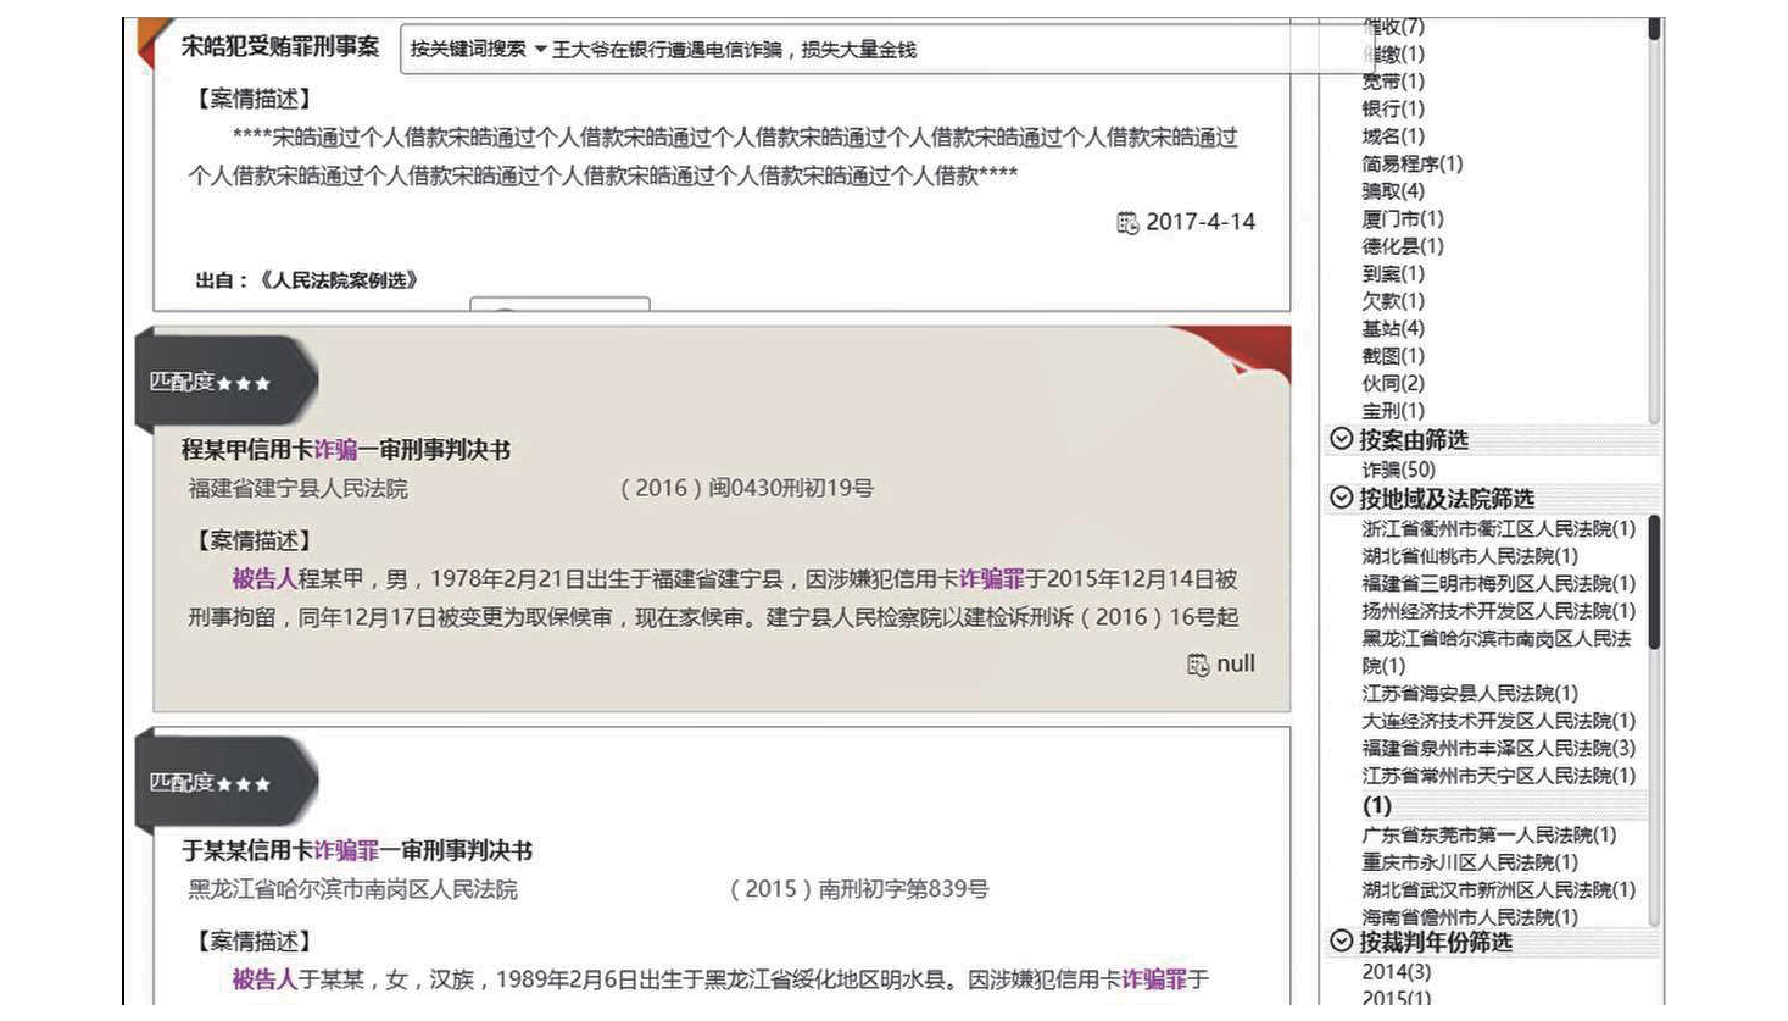
\includegraphics[scale=0.3, clip=true]{./sources/sys_search.eps}
    \caption{\label{fig:sys_search}个性化推荐功能展示图}
\end{figure*}

检索功能由输入功能框,检索结果,条件筛选三部分组成。当用户输入检索内容,通过章节~\ref{sec:sys_content}中语义相似度计算流程,展示出与检索内容相关的若干个裁判文书,并针对匹配得分的不同,展示匹配度信息。检索结果对裁判文书信息抽取后的信息进行结构化展示,并对与检索内容中的词语以及和这些词语有语义关联的词语进行高亮展示。条件筛选功能包含一些对裁判文书进行信息抽取后保存的结构化信息,通过点击这些结构化信息,用户可以进一步缩小范围,定位到所需要的内容。

输入功能框包含输入框,关键词关系图谱两个子功能,当用户输入查询,通过语义相似度计算模块,计算得到与检索内容中词语语义相关的词语,其结果如图~\ref{fig:sys_word}所示。
\begin{figure*}[htbp]%[htbp]
    \centering
    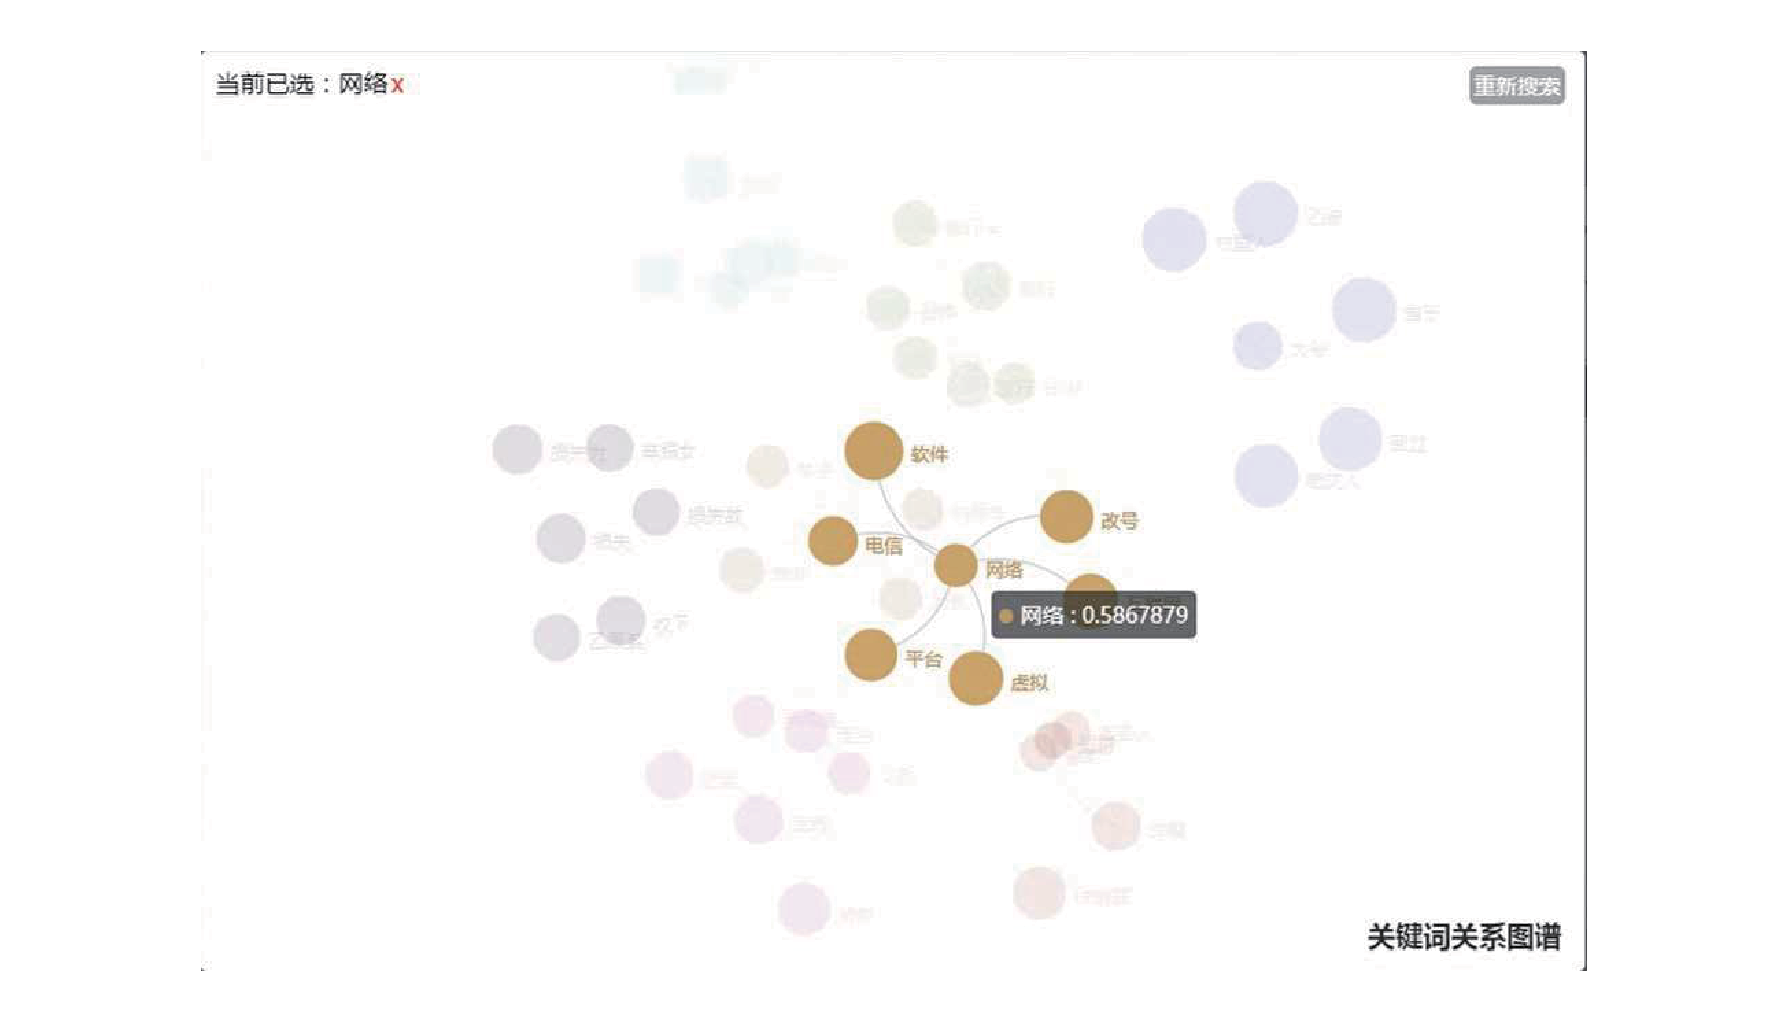
\includegraphics[scale=0.35, clip=true]{./sources/sys_word.eps}
    \caption{\label{fig:sys_word}关键词关系图谱功能展示图}
\end{figure*}

\subsection{判决预测功能测试}
判决预测功能由输入框与预测结果两部分组成。当用户在输入框输入检索内容,经过本课题第三章和第四章模型计算,预测得到与检索内容相关的法条信息,结果如图~\ref{fig:sys_article}所示。
\begin{figure*}[htbp]%[htbp]
    \centering
    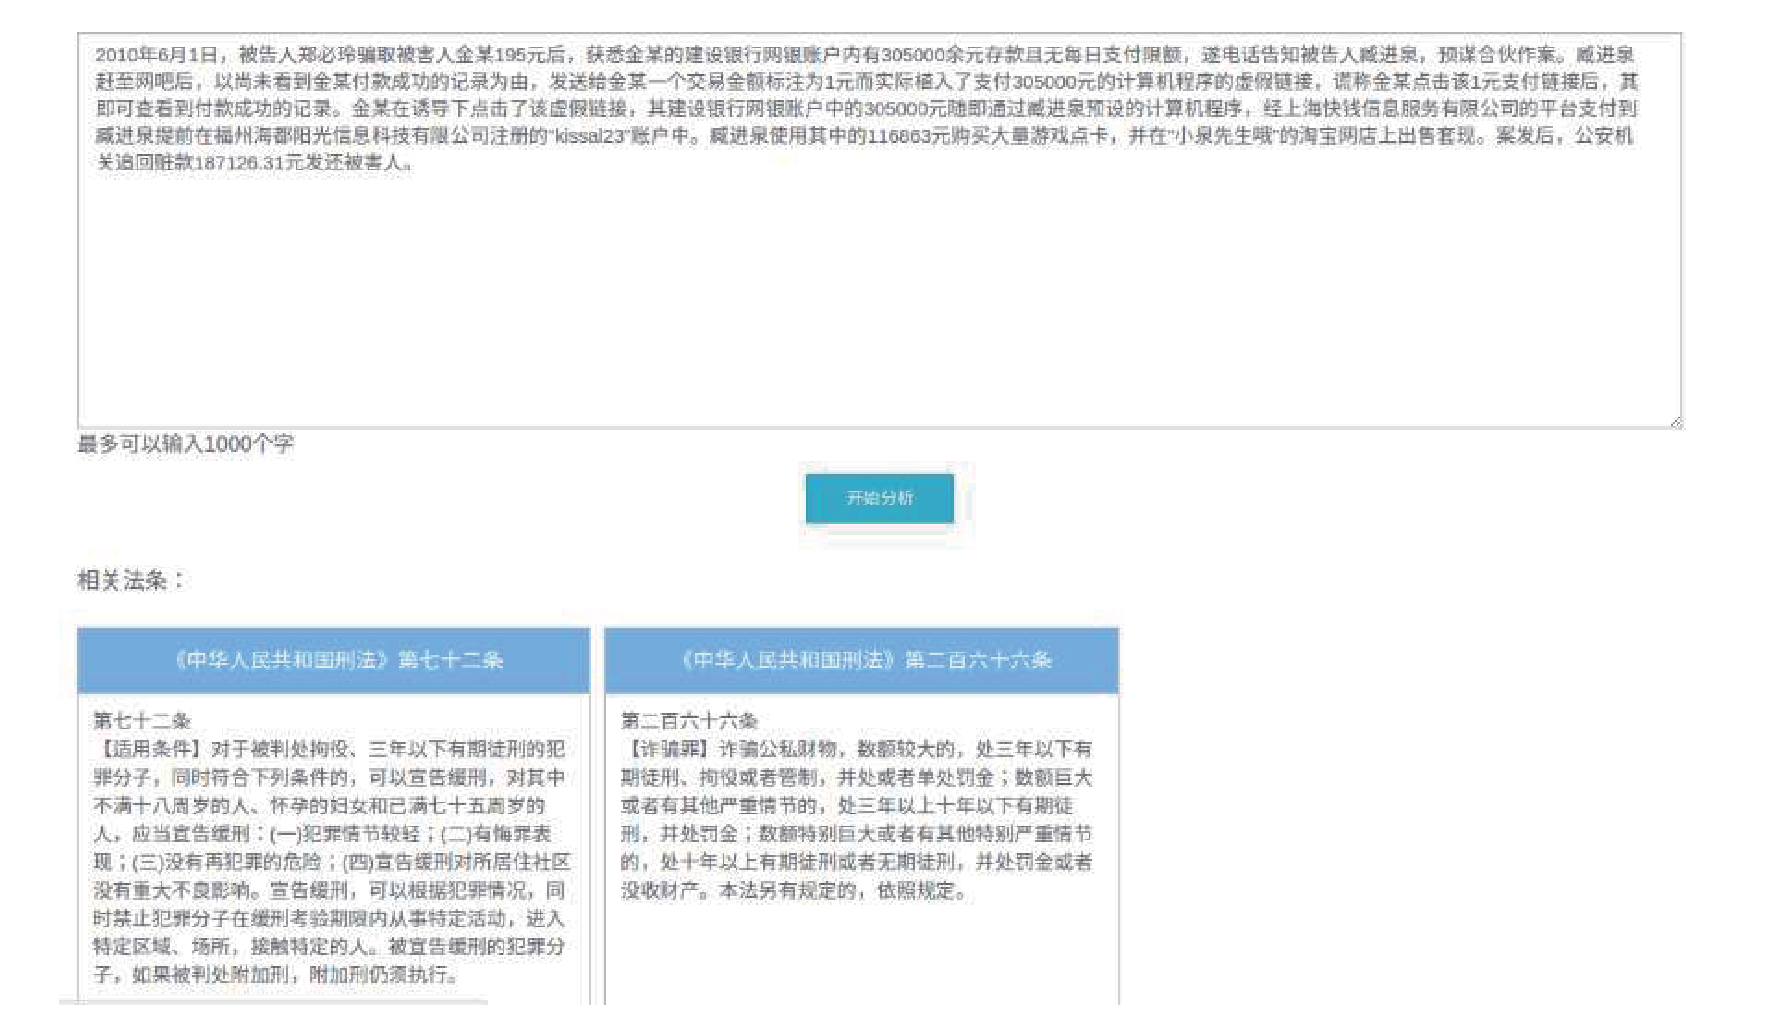
\includegraphics[scale=0.35, clip=true]{./sources/sys_article.eps}
    \caption{\label{fig:sys_article}法条预测功能展示图}
\end{figure*}

\section{本章小结}
本章对本课题研究内容的实际落地原型系统进行了介绍,首先介绍了系统功能设计,对原型系统的整体框架分模块进行了介绍,之后对原型系统类案检索功能与判决预测功能进行了测试,使本课题研究模型算法在系统中进行有效应用。